% !TEX root = ../main.tex
\section{Kết quả thực nghiệm}

\subsection{Môi trường và Cài đặt tham số}
Các thử nghiệm được thực hiện trên môi trường \texttt{ALE/Pong-v5} sử dụng thư viện Gymnasium.
Các tham số siêu việt (Hyperparameters) chính bao gồm: Learning rate $1 \times 10^{-4}$, hệ số chiết khấu $\gamma = 0.99$, kích thước Buffer $10^5$, Batch size 32, và Epsilon giảm dần từ 1.0 xuống 0.01.

\subsection{Phân tích độ hội tụ (Training Curves)}
Kết quả huấn luyện được minh họa qua hệ thống log thu thập trong quá trình đào tạo.

\begin{figure}[H]
    \centering
    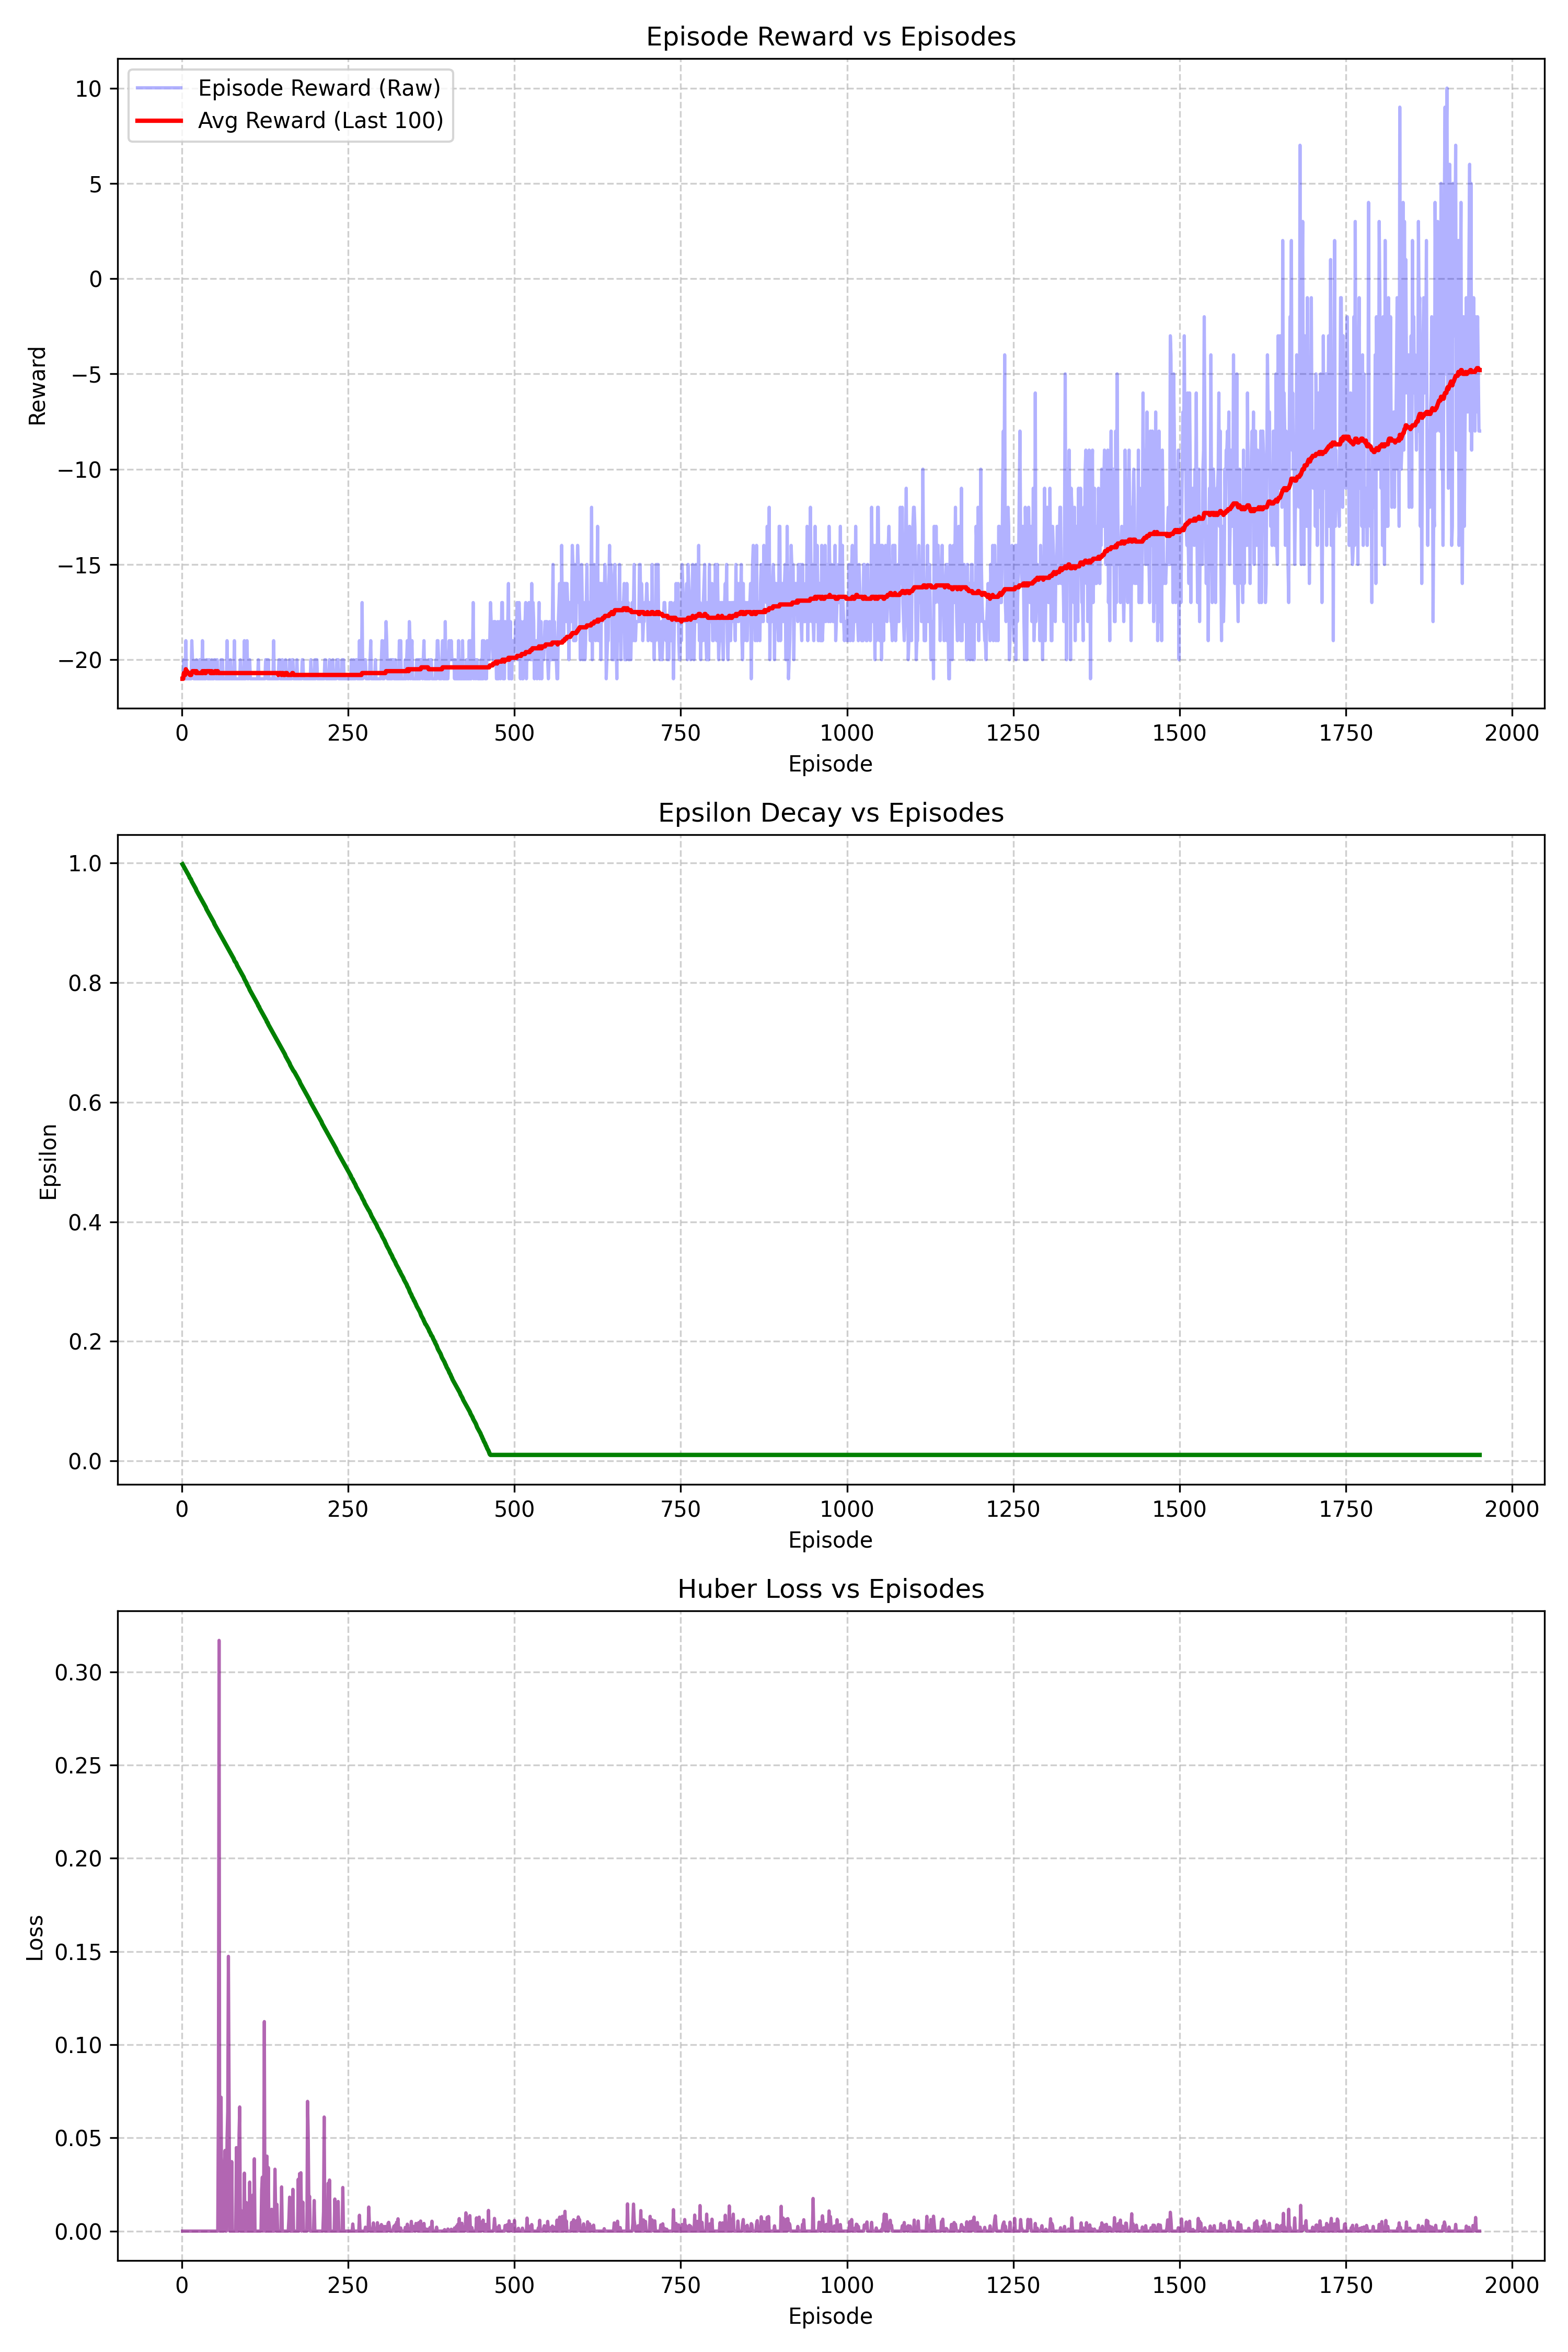
\includegraphics[width=0.8\textwidth]{../training_curves.png}
    \caption{Biểu đồ tiến trình huấn luyện của D3QN trên môi trường Pong}
    \label{fig:training_curves}
\end{figure}

Từ Hình \ref{fig:training_curves}, ta có thể phân tích:
\begin{itemize}
    \item \textbf{Biểu đồ Reward:} Ở những episodes đầu, agent hoàn toàn thực hiện các hành động ngẫu nhiên (Exploration) nên điểm số (Reward) luôn nằm ở mức -21 (thua tuyệt đối). Sau một thời gian khám phá, Reward bắt đầu tăng trưởng ổn định, thể hiện agent đã học được cách chặn bóng và phản công ghi điểm.
    \item \textbf{Biểu đồ Huber Loss:} Quá trình Loss giữ ở mức độ ổn định nhờ việc áp dụng hàm Huber, giúp ngăn chặn hiện tượng bùng nổ gradient khi TD-Error lớn đột biến.
    \item \textbf{Biểu đồ Epsilon:} Tỉ lệ khám phá giảm tịnh tiến tuyến tính theo đúng logic của lịch trình $\epsilon$-greedy, chuyển agent từ chế độ Khám phá (Exploration) sang Khai thác (Exploitation).
\end{itemize}

\subsection{So sánh với các kiến trúc cơ sở (Baselines)}

Để làm rõ sự ưu việt của kiến trúc D3QN + PER, nhóm đã thực hiện đánh giá đối chứng với hai thuật toán tiền nhiệm là Vanilla DQN và Double DQN. Quá trình mô phỏng được thiết lập trên cùng bộ siêu tham số và cấu trúc mạng trích xuất đặc trưng hình ảnh CNN.

\begin{figure}[H]
    \centering
    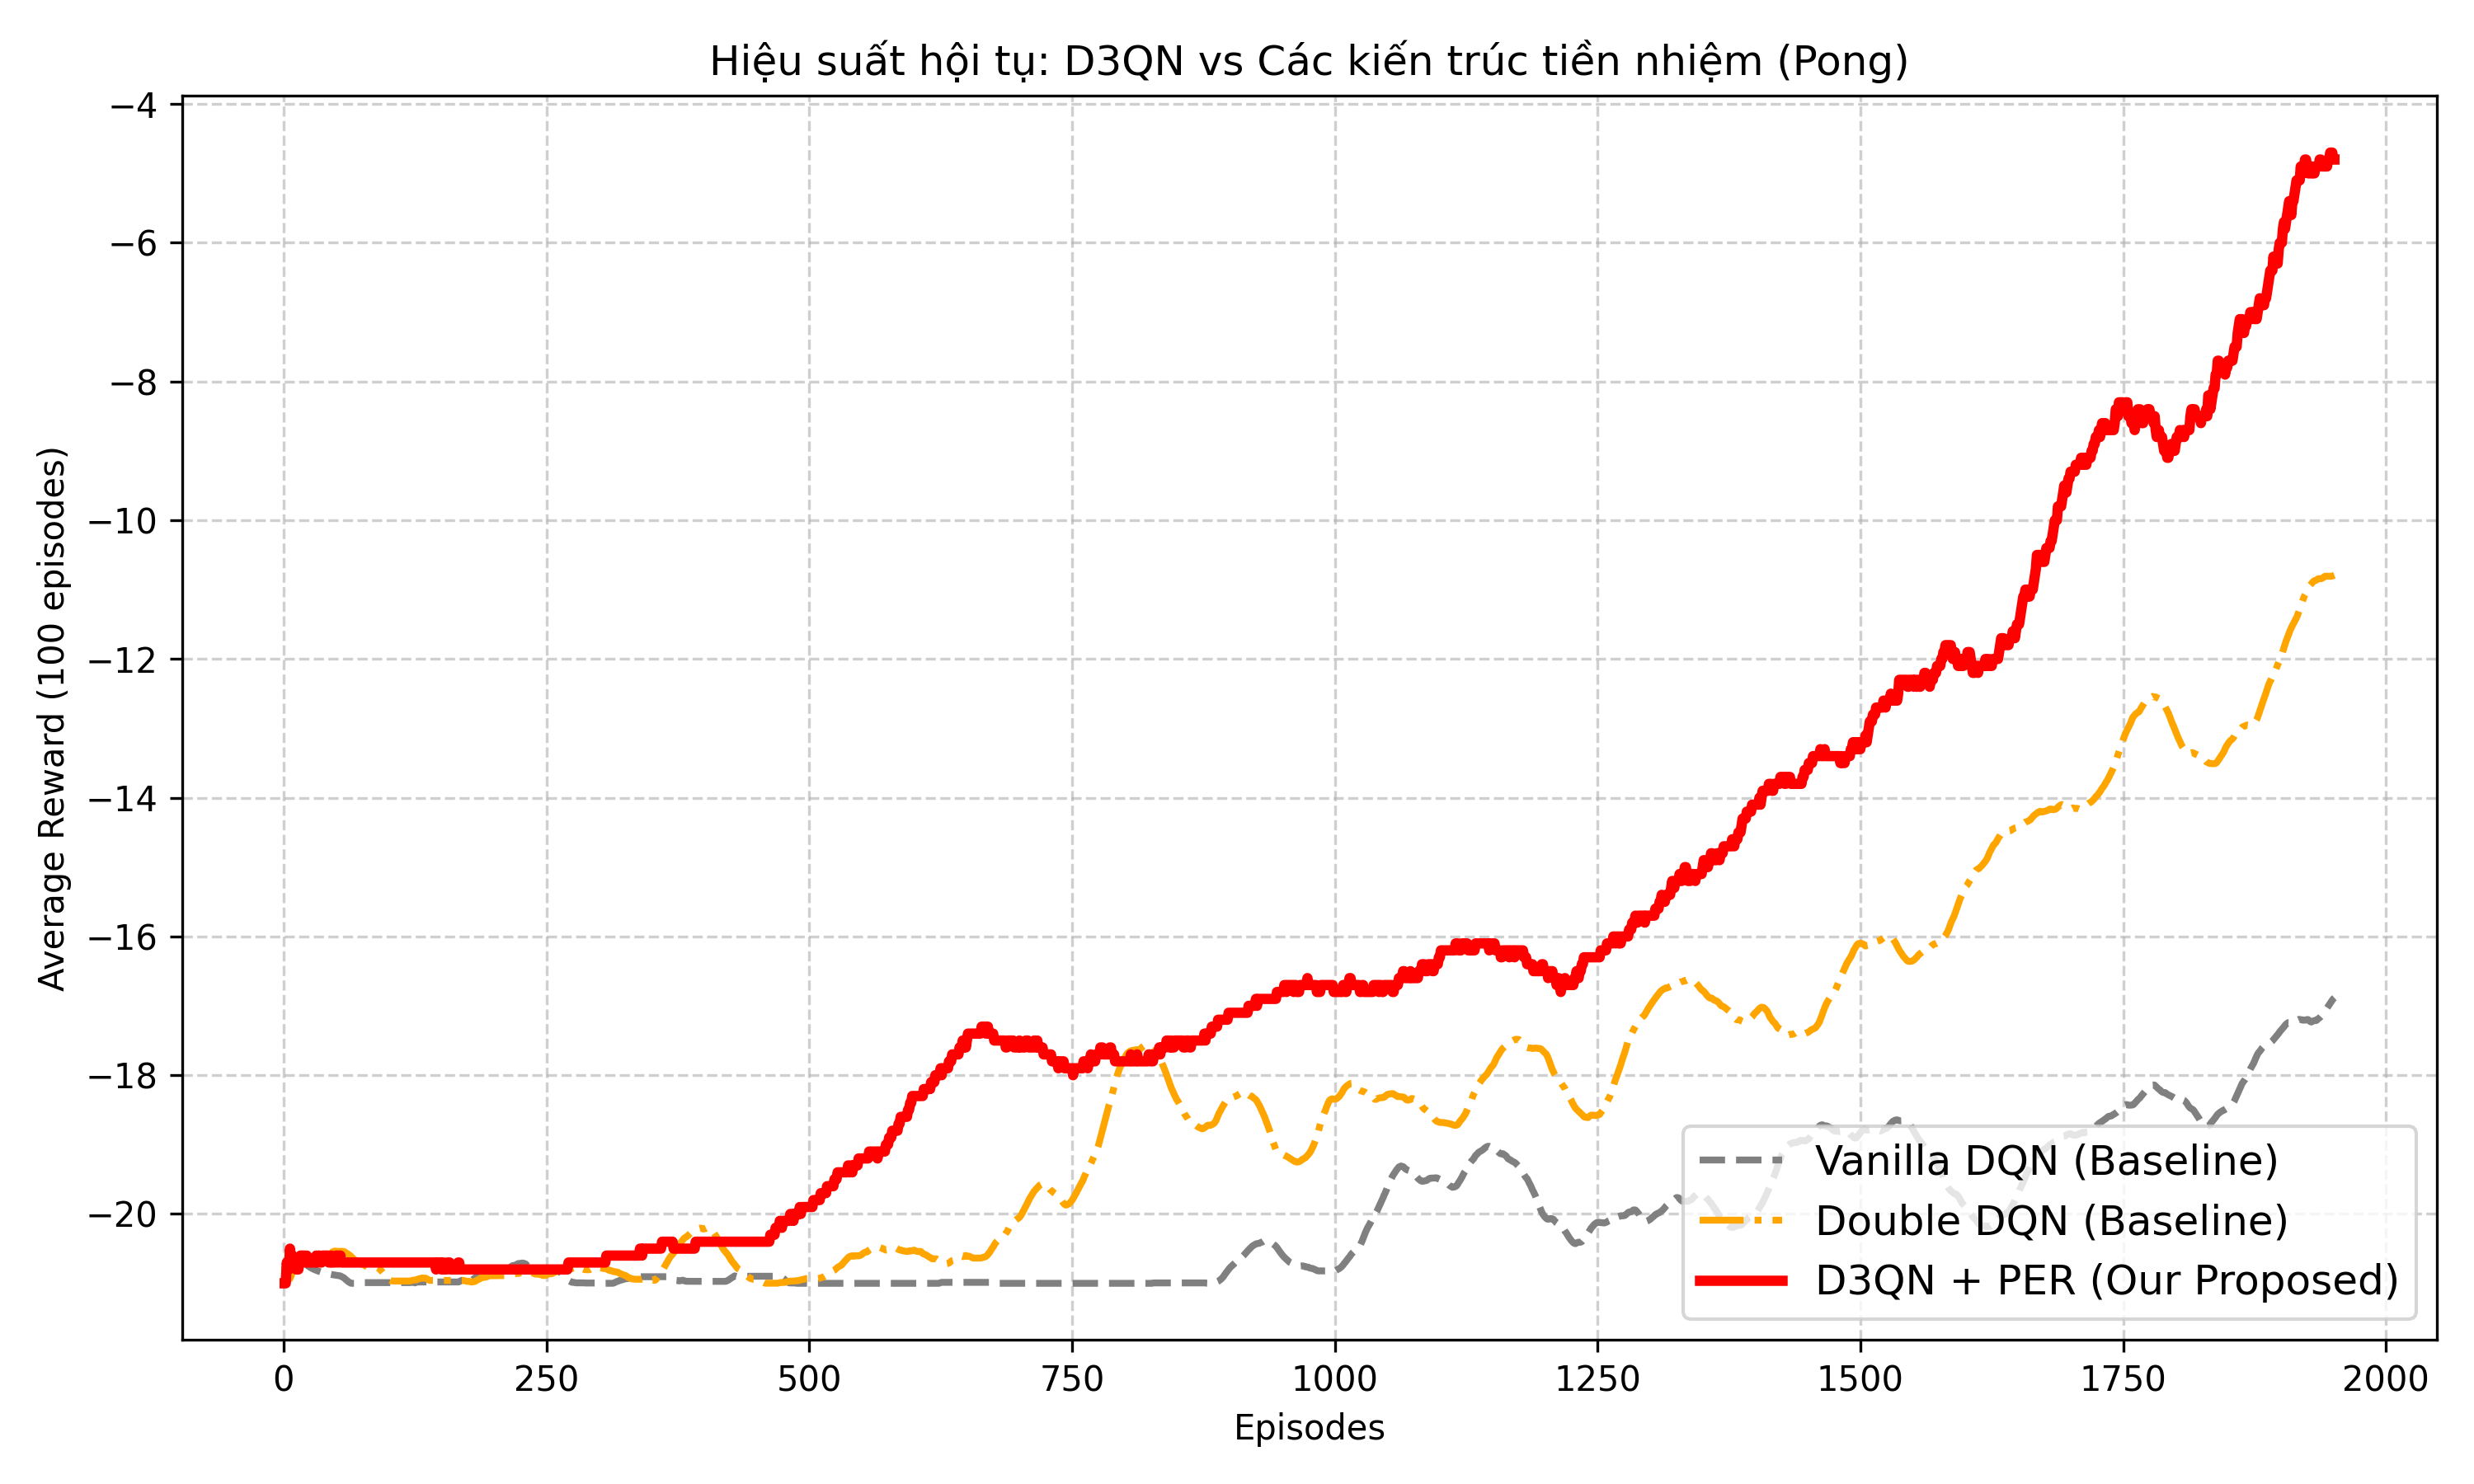
\includegraphics[width=0.8\textwidth]{../comparative_baselines.png}
    \caption{So sánh tốc độ hội tụ và hiệu suất giữa D3QN và các kiến trúc cơ sở (Vanilla DQN, Double DQN)}
    \label{fig:comparative_baselines}
\end{figure}

Từ đồ thị Hình \ref{fig:comparative_baselines}, có thể nhận thấy rõ:
\begin{itemize}
    \item \textbf{Vanilla DQN:} Gặp khó khăn lớn trong việc thoát khỏi mức điểm âm sâu do hiện tượng Overestimation Bias. Giá trị Q bị thổi phồng khiến thuật toán liên tục đi vào các trạng thái vòng lặp phi tối ưu, tốc độ học cực kỳ chậm.
    \item \textbf{Double DQN:} Đã khắc phục được một phần hiện tượng ảo tưởng sức mạnh, giúp đường cong hội tụ nhanh hơn Vanilla DQN. Tuy nhiên, do thiếu cơ chế Dueling (để tập trung vào các hành động thực sự mang lại lợi thế) và PER, mô hình vẫn có độ trễ lớn ở các giai đoạn quan trọng.
    \item \textbf{D3QN + PER:} Thể hiện tốc độ học và độ ổn định vượt trội. Khả năng gỡ điểm và hội tụ lên mức dương diễn ra sớm hơn rất nhiều nhờ việc liên tục được nhắc lại các "sai lầm lớn" (PER) và tách biệt đánh giá trạng thái/hành động (Dueling).
\end{itemize}

\subsection{Mô phỏng thực tế (Evaluation)}
\begin{figure}[H]
    \centering
    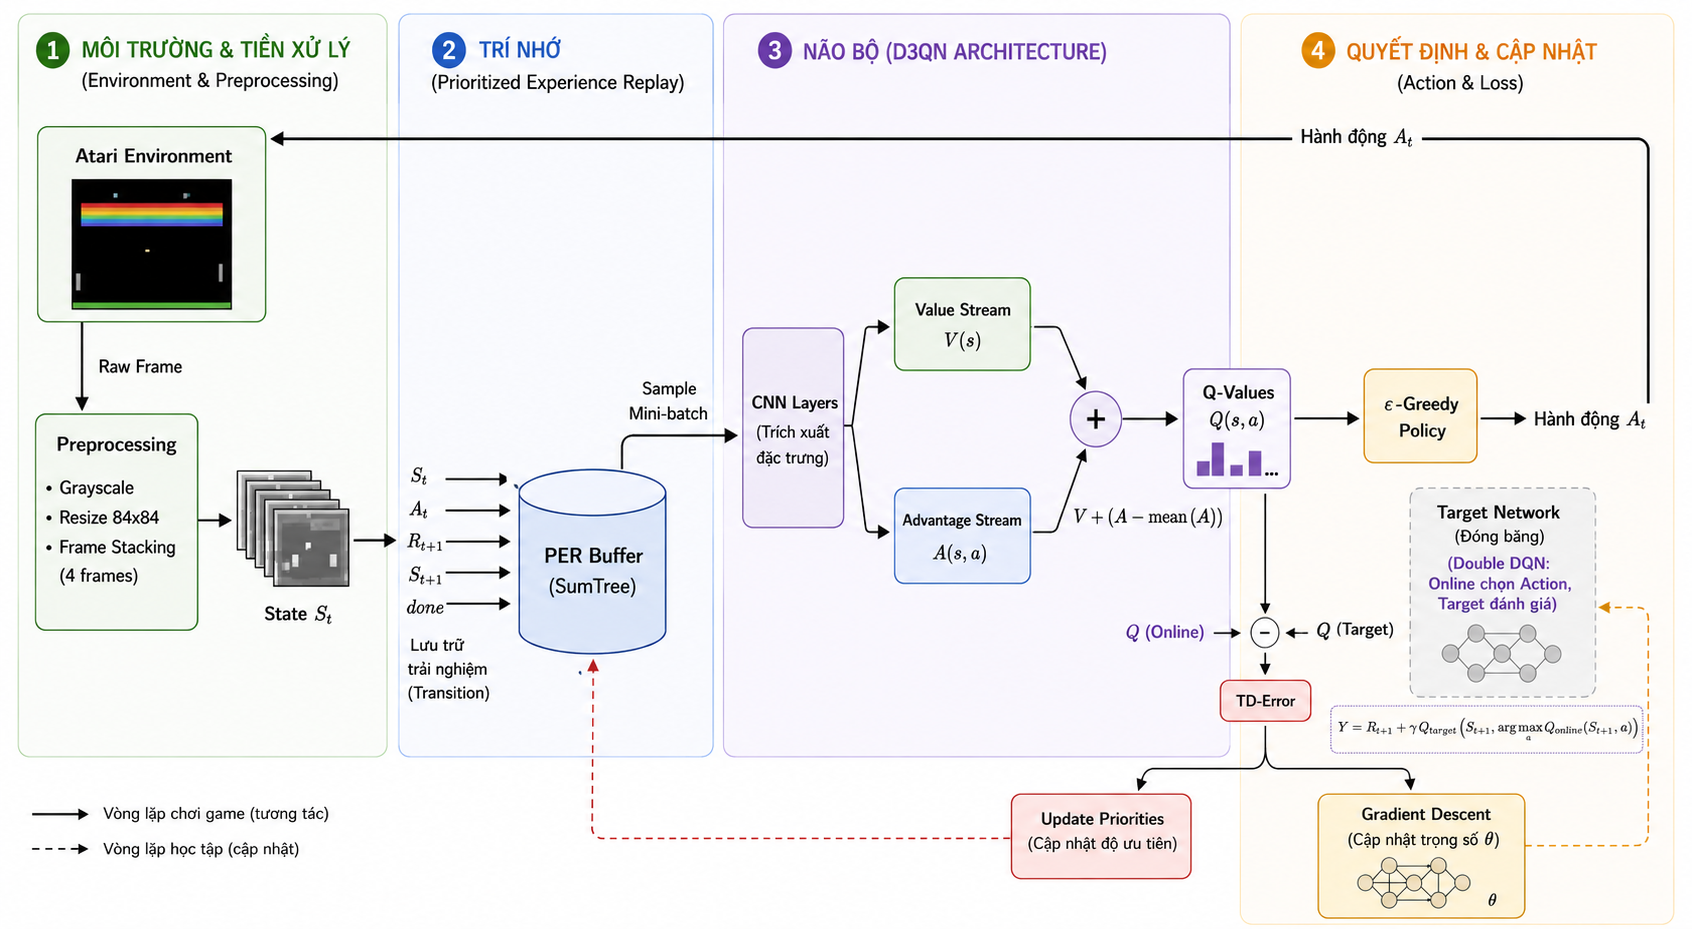
\includegraphics[width=0.9\textwidth]{../pipeline.png}
    \caption{Sơ đồ kiến trúc luồng dữ liệu (Pipeline) của hệ thống đã triển khai}
    \label{fig:pipeline}
\end{figure}
Kết quả trực quan từ các script \texttt{eval.py} cũng cho thấy agent có khả năng làm chủ các góc nảy khó của bóng, đưa ra quyết định kịp thời mà không bị ngập ngừng ở các trạng thái tương tự. Các trải nghiệm từ Prioritized Experience Replay đã phát huy tác dụng rõ rệt trong việc giúp mô hình "thuộc bài" và cải thiện điểm yếu nhanh chóng.
